\chapter{IRRADIANCE MONITORING NETWORK}
\label{chap:sens_net}

Using historical data from 80 residential rooftop PV systems, Lonij
\etal produced intra-hour solar power forecasts that showed skill over
persistence forecasts \citep{Lonij2013}.
The local electric utility, Tucson Electric Power (TEP), was interested in
receiving these short-term forecasts in real-time.
To generate real-time forecasts, data from sensors need to be gathered
in real-time
Thus we set out building the irradiance monitoring network described
in this chapter that would report values in near real-time.
To accomplish this goal, we designed custom irradiance sensors that
are deployed remotely and report data in real-time via cell model as
described in \cref{sec:custom_sensors}.
We also partnered with a local rooftop PV installer to gather power
data from PV systems to act as proxies for irradiance, described in
\cref{sec:pv_sensors}.
This irradiance monitoring network, that was deployed in Tucson, AZ, is
the basis for much of the forecasting work in this dissertation.


\section{Design of Custom Sensors}
\label{sec:custom_sensors}
This section describes the custom irradiance sensors that were
developed to support the forecasting work in this dissertation.
These sensors were custom designed based upon the lack of available,
low-cost alternatives.
The sensors as described cost around \$500 in raw materials when they
were built in early 2014.
This low cost allowed us to build and deploy many sensors to collect
more data.
The sensors were also designed to communicate data back in real-time
so that the network could be used to produce operational forecasts for
TEP.

\subsection{Photodiode Sensor}
\label{sec:photodiode}
A number of photodiodes were studied to determine a suitable,
inexpensive replacement for a pyranometer to measure irradiance.
We tested a clear domed photodiode which we sanded to better diffuse
light, a thin sheet of Teflon glued on a photodiode to diffuse light,
and a an unmodified, flat photodiode, among others.
We found that the flat photodiode (Osram BPW34) provided a reasonable
signal level and cosine response, shown in \cref{fig:pdshape}.
This photodiode is sufficient to detect deviations in the irradiance from
clear-sky conditions, as a pyranometer would, which is the main way
the network is used.

\begin{figure}[h]
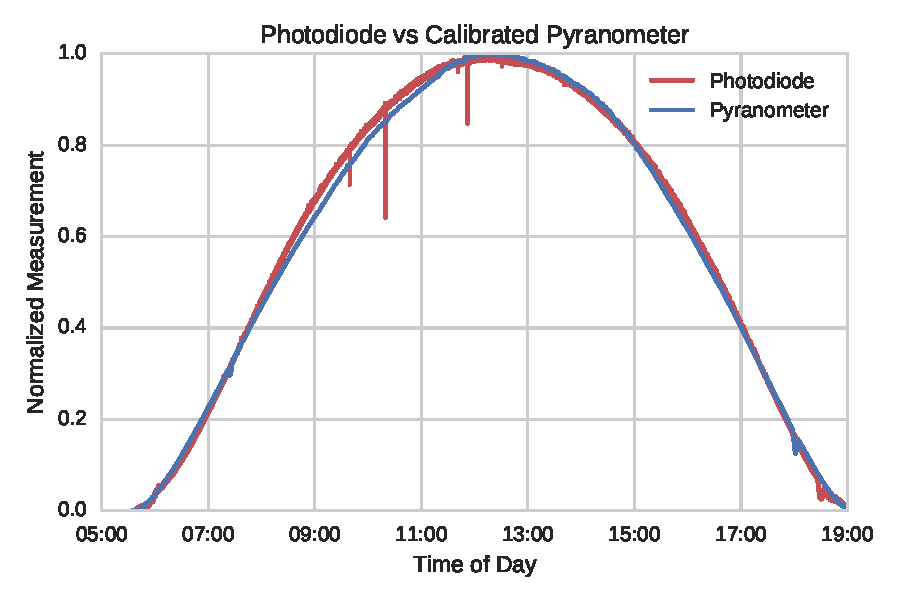
\includegraphics[width=\textwidth]{figs/pdvspy.pdf}
\caption[Comparison of photodiode and pyranometer signals]{A
  comparison of the signal from a photodiode and a calibrated
  pyranometer. The photodiode does not exhibit a perfect cosine
  response with a wider peak that decays too quickly. However, the
  photodiode performs well for the main purpose of detecting changes
  in irradiance. Note that the noise in the measurement of the
  photodiode is about double the noise in the pyranometer measurement.}
\label{fig:pdshape}
\end{figure}

\subsection{Hardware}
\label{sec:senshardware}
A custom printed circuit board was designed for the components that
store and send sensor data to a central server every minute.
The circuit diagram for this board is shown in \cref{fig:circuit}.
Design files for the circuit board can be found online~\cite{Lorenzo2017a}.

\begin{sidewaysfigure}[p]
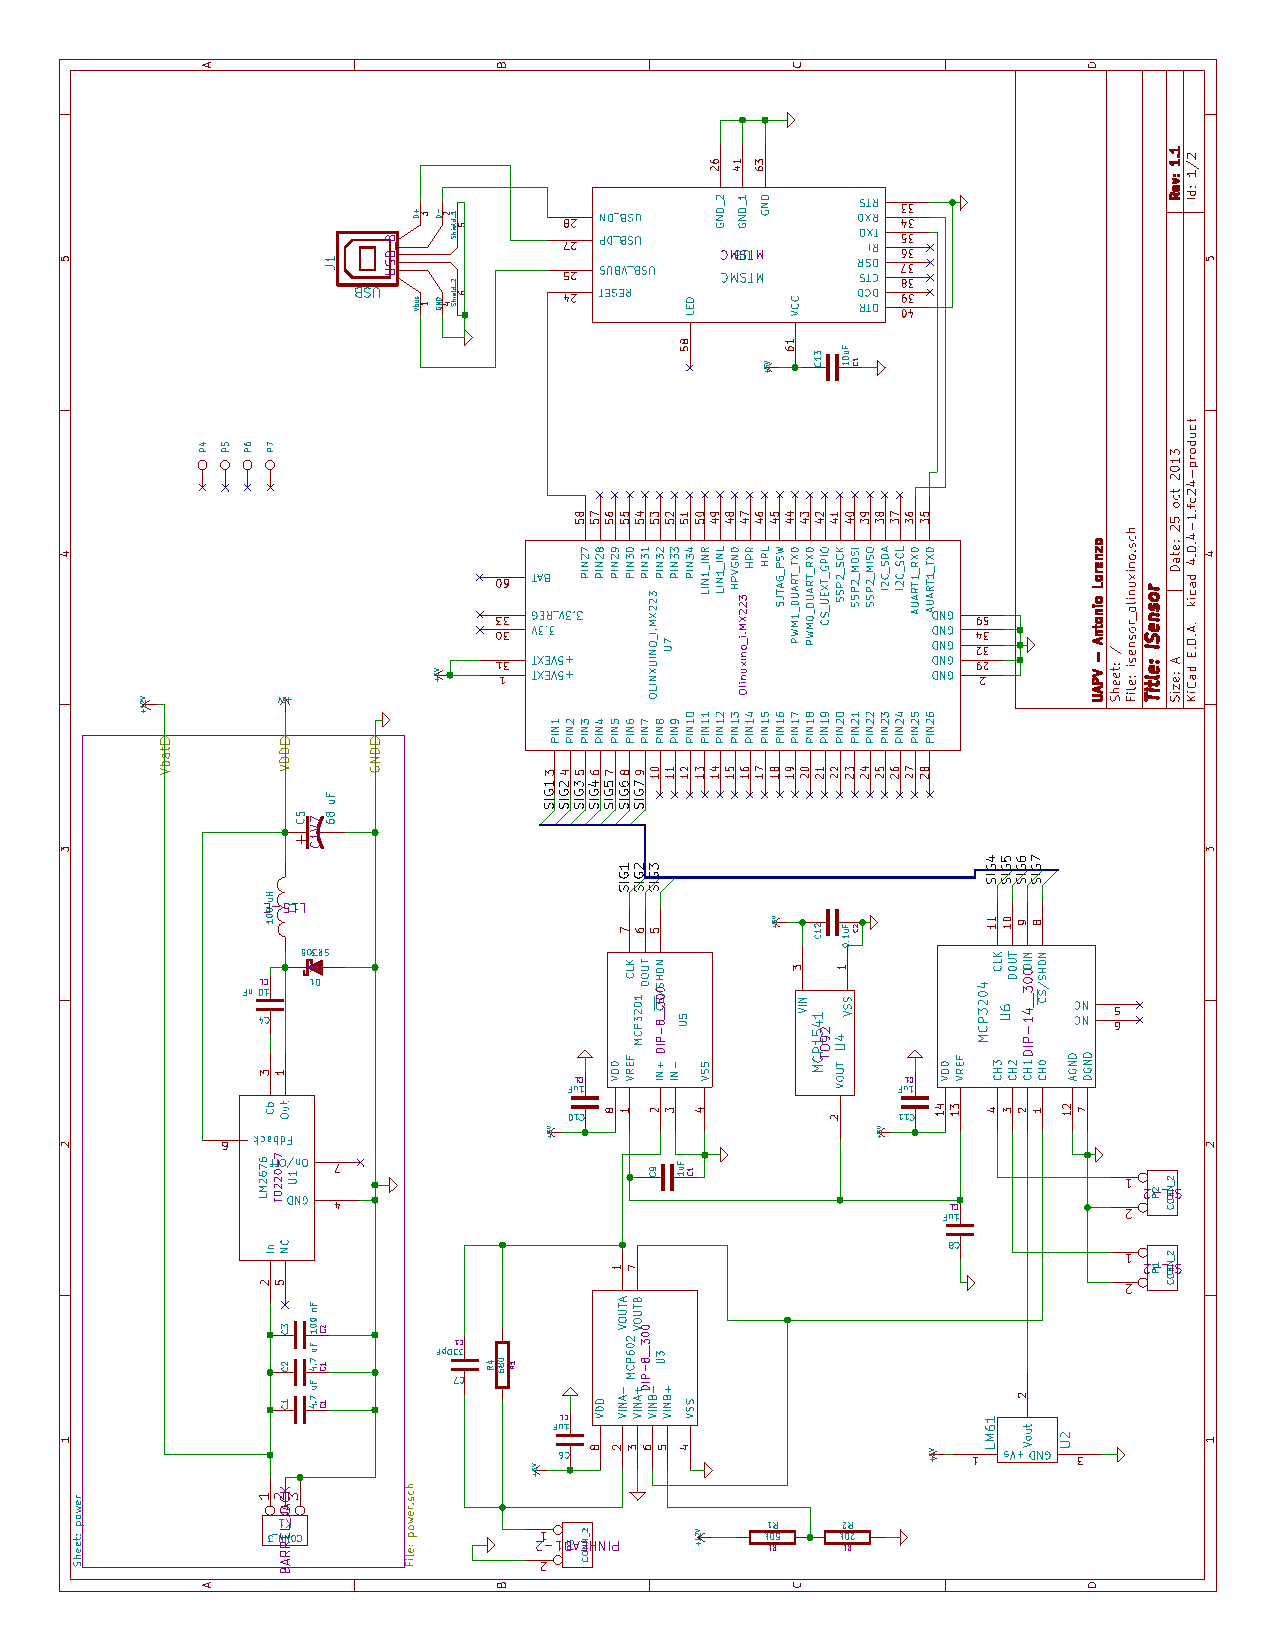
\includegraphics[angle=-90,width=\textwidth]{figs/circuit.pdf}
\caption[Custom sensor circuit diagram]{Circuit diagram for the
  custom, remote irradiance sensors. See \cref{sec:senshardware} for a
  description of the components.}
\label{fig:circuit}
\end{sidewaysfigure}

The custom sensors are developed around the Olimex
iMX223-OLinuXino-MICRO board.
The OLinuXino was chosen because it consumes little power ($< 1$W) and it
runs a full Linux operating system which allows for development in any
language that can be installed on Linux along with the usual suite of
Linux tools (SSH, Bash, logs).
It is also relatively inexpensive to purchase complete boards, and the
plans are open-source if one desires to build the board themselves.

Data is communicated via GSM using a MULTITECH MTSMC-H5-U SocketModem.
This modem accepts a standard SIM card that is registered with a
cellular data provider.
The modem is connected to the OLinuXino via USB.
WvDial and PPPD are used to setup the connection to the modem and
allow internet access.

Power to the system is provided by a 10W solar panel and a 6Ah
lead-acid battery.
A standard solar charge controller is used limit the current from the
panel to the battery.
The nominal 12V from the battery is routed to the circuit board with
the OLinuXino and modem and converted to 5VDC with a circuit based on
the LM2676 step-down regulator.

The sensor is designed to accept input from either a calibrated
pyranometer (Apogee SP-212) or an inexpensive silicon photodiode
(Osram BPW34) as discussed in \cref{sec:photodiode}.
A trans-impedance amplifier (MCP602) with appropriate gain is used to
convert the current from the photodiode into a measurable voltage.

The voltage from the sensor (or sensor + trans-impedance amplifier) is
converted to a digital signal with the MCP3201 12-bit
analog-to-digital converter (ADC).
This digital signal is then read the OLinuXino at regular intervals
from the GPIO pins.
An additional 4 channel 12-bit ADC (MCP3204) is used to convert other
values such as enclosure temperature (measured by an LM61) and battery
voltage to be read on the OLinuXino GPIO pins for monitoring.
A 4.096V voltage reference (MCP1541) is used by both ADCs.

\begin{figure}[t]
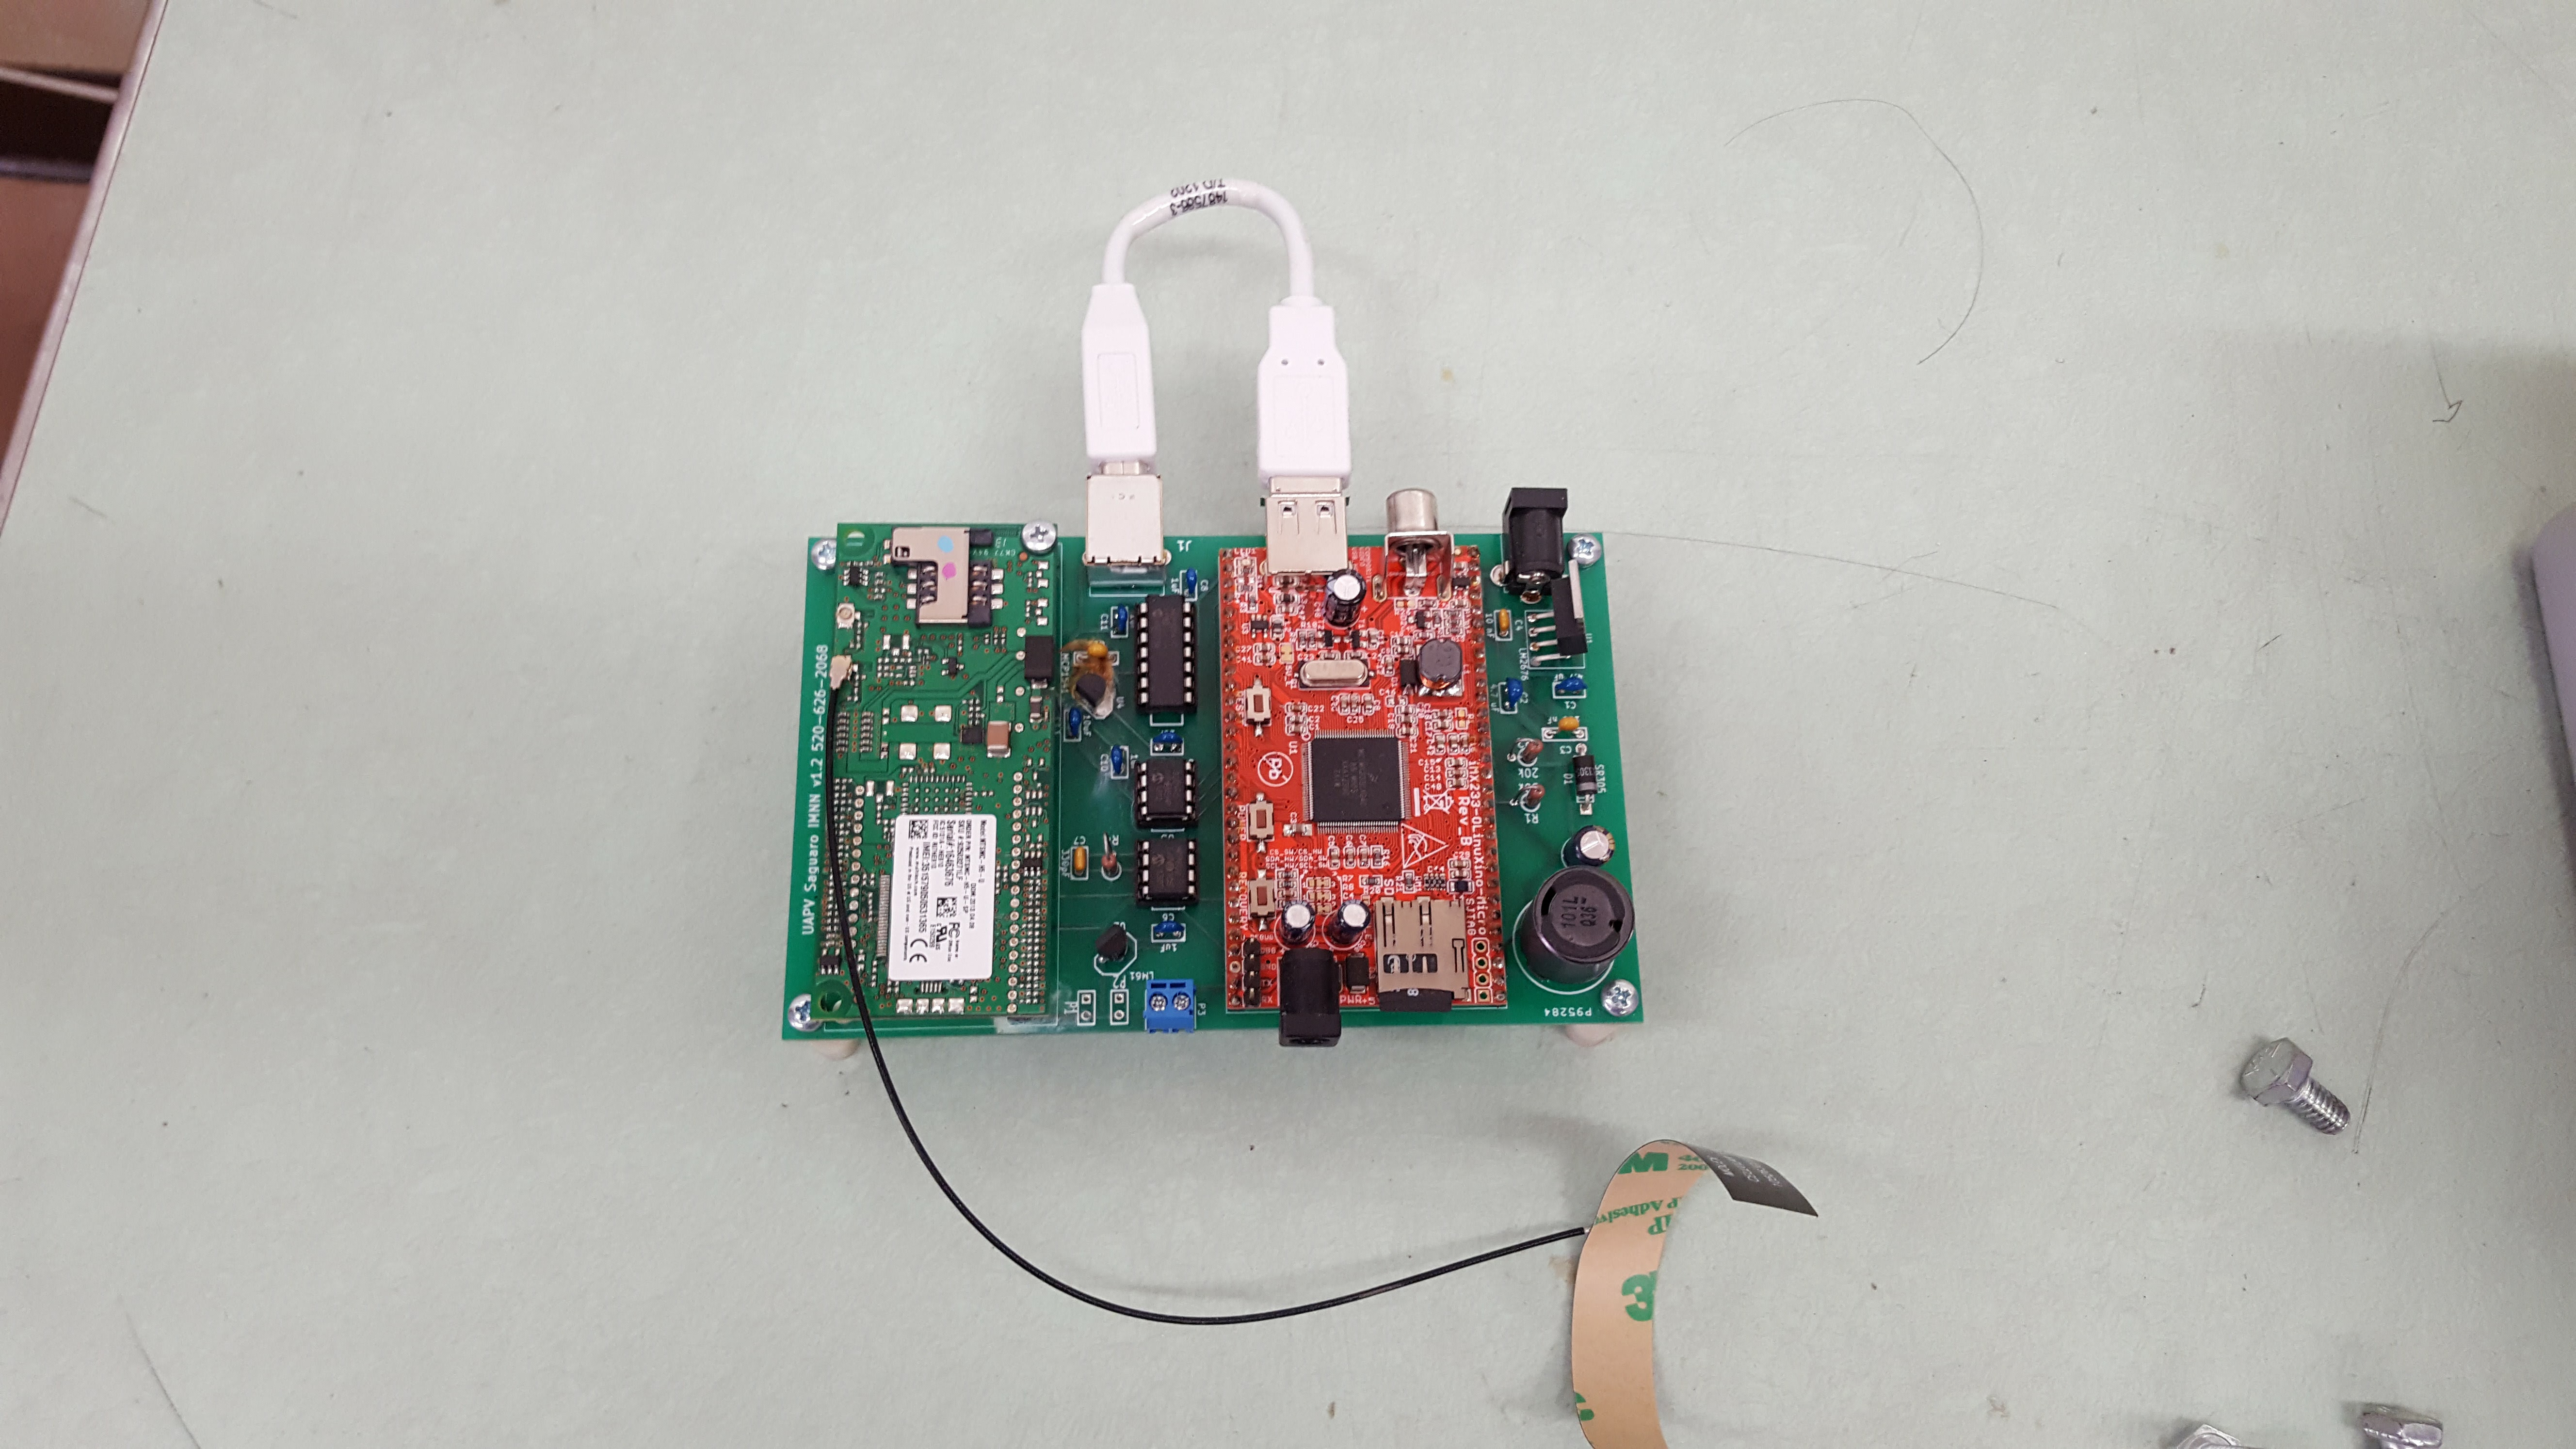
\includegraphics[width=\textwidth]{figs/sensor_board.jpg}
\caption[Assembled sensor circuit board]{A fully assembled printed
  circuit board for a custom sensor. The red board is the OLinuXino
  and the green board on the left is the cell modem with a flexible
  antenna. Through hole components were chosen for easy soldering.}
\label{fig:sensor_board}
\end{figure}

A fully assembled printed circuit board is shown in
\cref{fig:sensor_board}.
The circuit board is housed in a waterproof box with an air snorkel
and cable nipples to maintain water resistance.
A metal extrusion serves as a mast to mount the photodiode or
pyranometer.
The solar panel and this mast are attached to the top of the
waterproof box which can then be placed outside.
A photo of the interior of the box with the circuit board and lead
acid battery is shown in \cref{fig:sensor_int}.
An entire completed sensor undergoing testing is shown in
\cref{fig:sensor_outside}.

\begin{figure}[ht]
  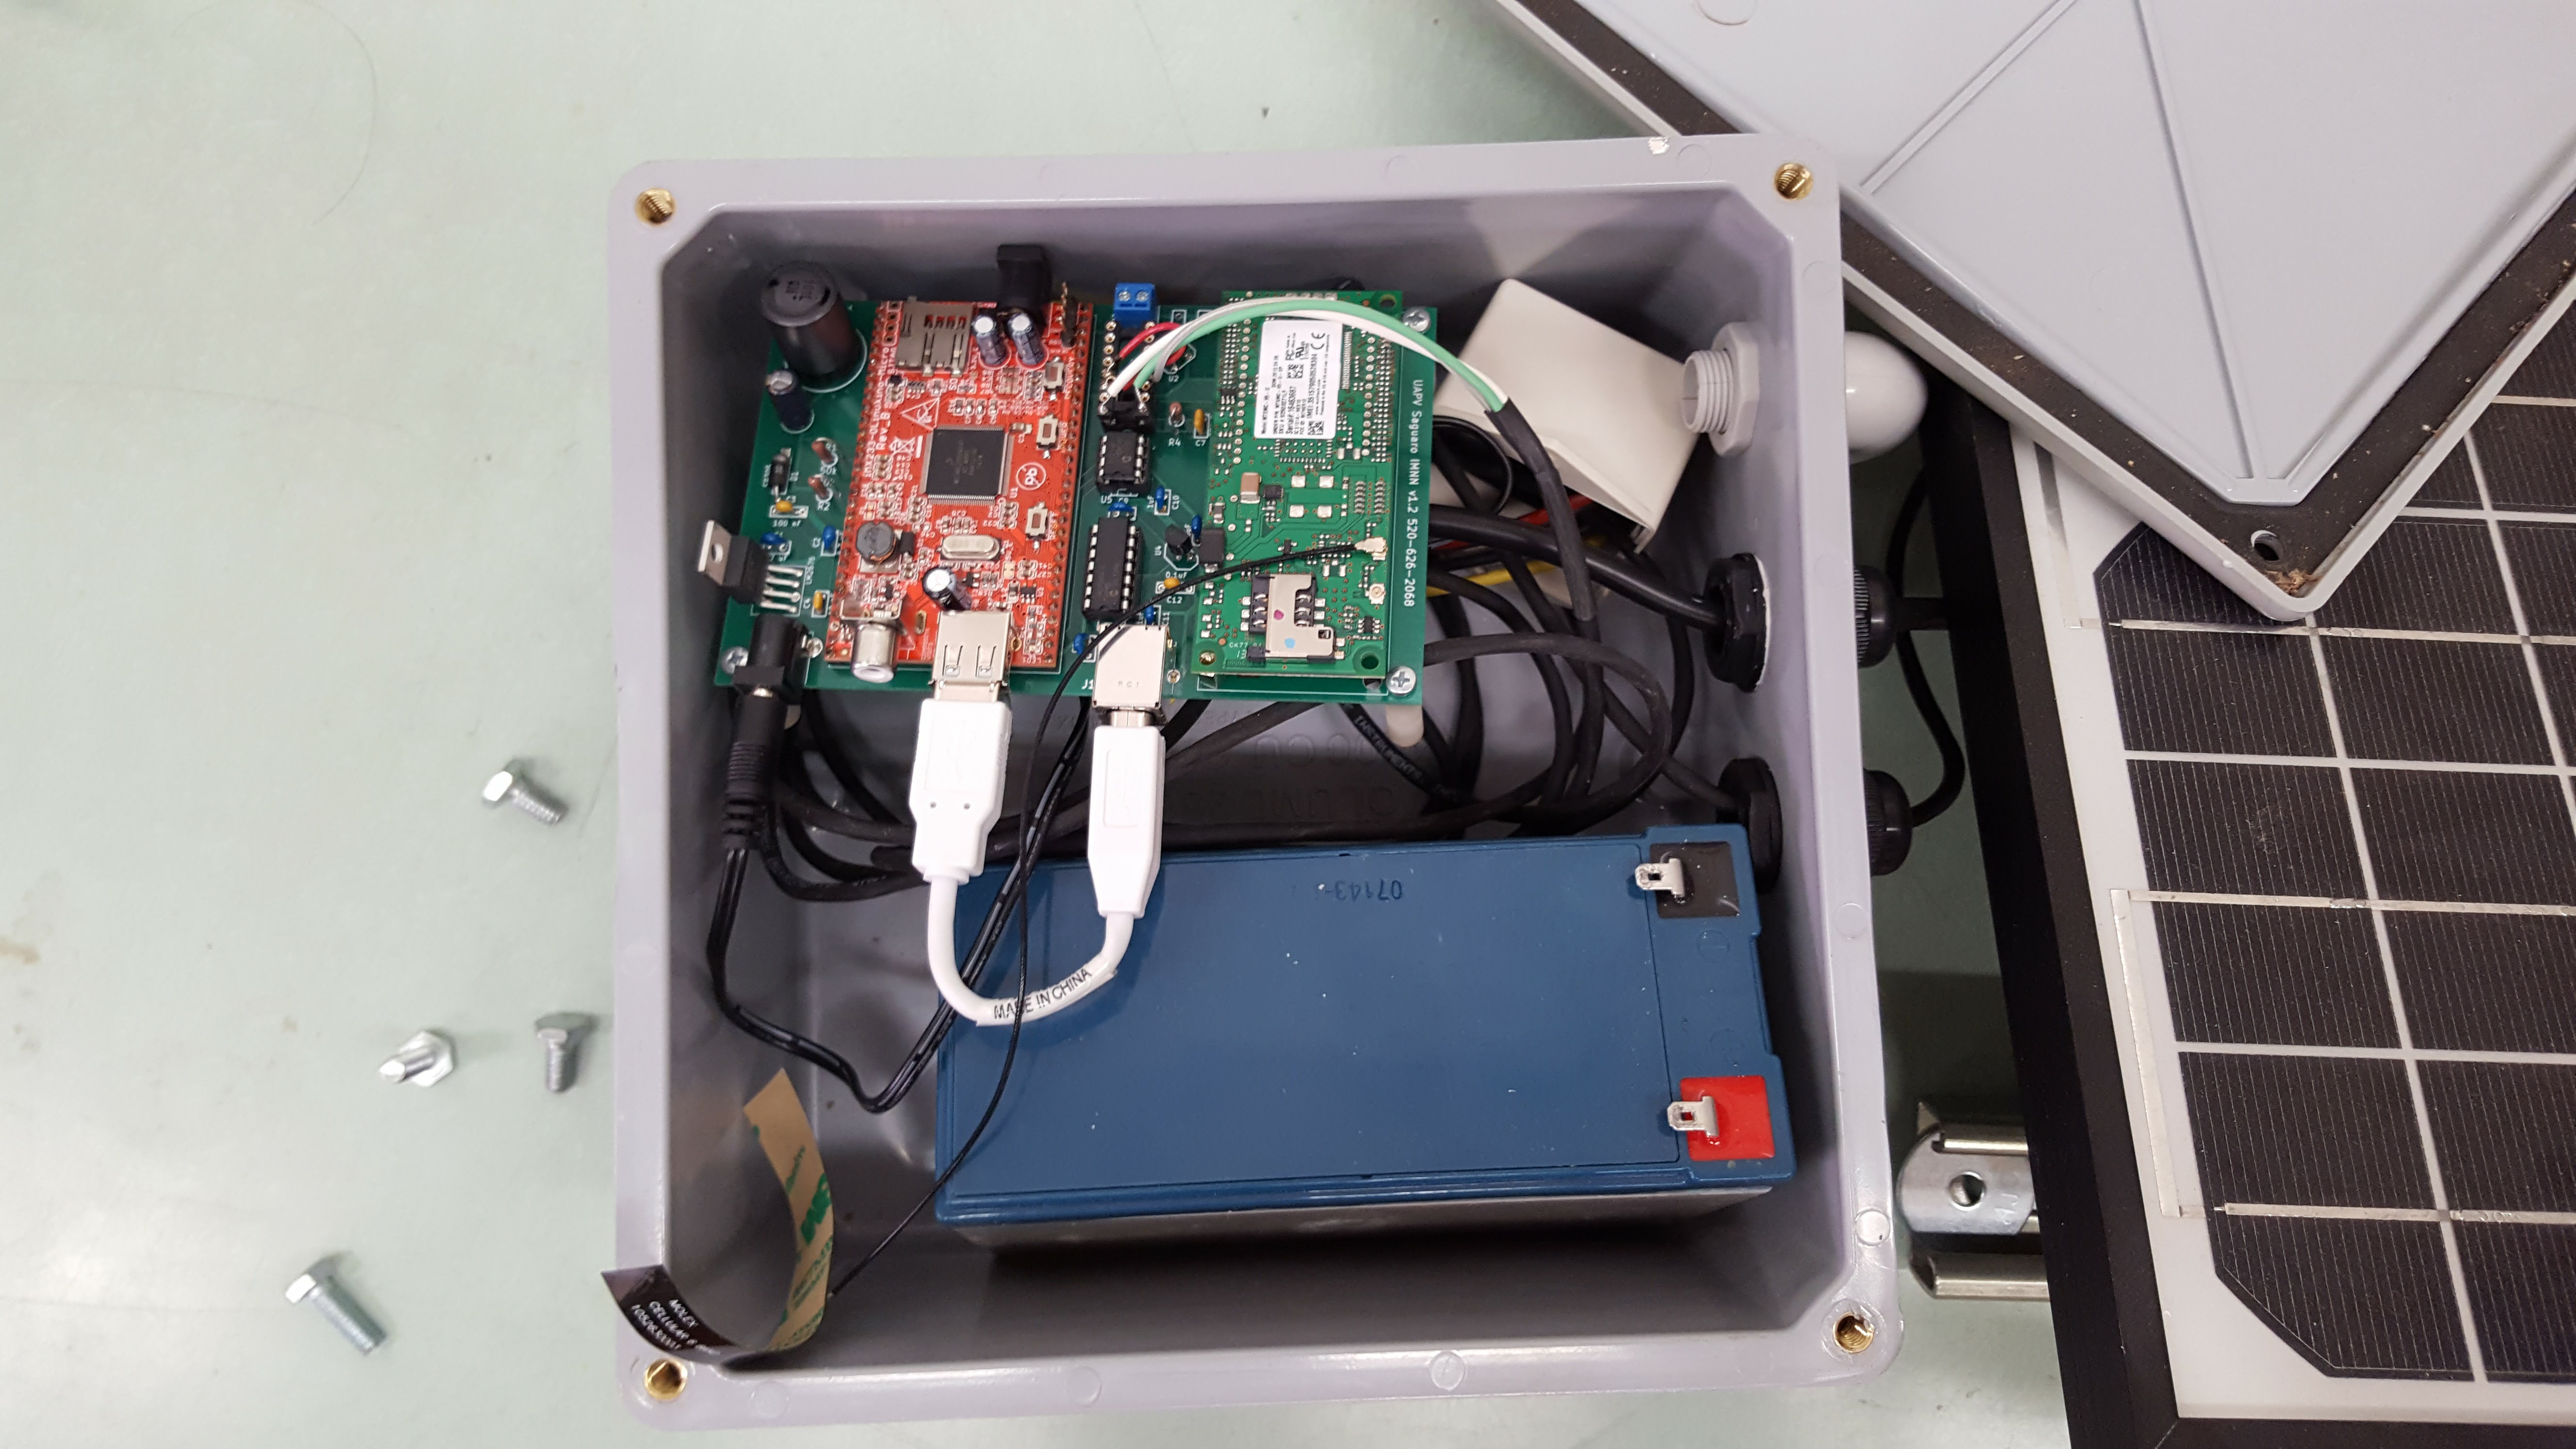
\includegraphics[width=\textwidth]{figs/sensor_interior.jpg}
\caption[Interior of the sensor enclosure]{A photo of the interior of
  the sensor enclosure. The air vent and waterproof cable nipples are
  visible on the right side of the box. The 6Ah 12V motorcycle battery
  is shown near the bottom.}
\label{fig:sensor_int}
\end{figure}

\begin{figure}[p]
  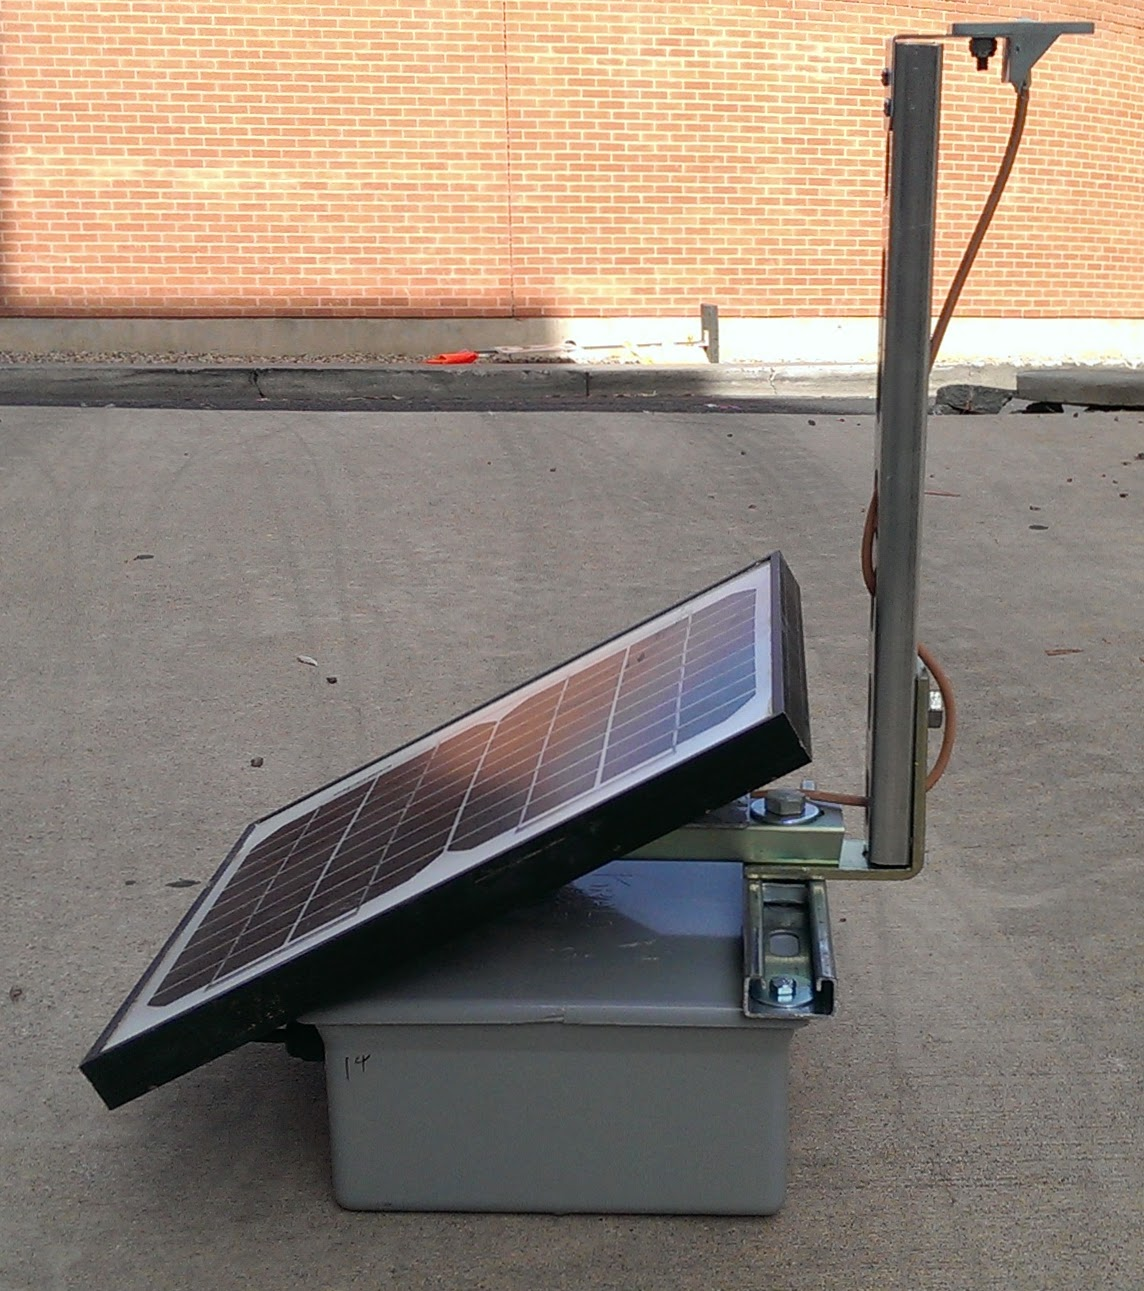
\includegraphics[width=\textwidth]{figs/sensor_outside.jpg}
\caption[A complete custom sensor]{A photo of a complete custom
  irradiance sensor as it undergoes testing outside. The photodiode
  sensor can be see mounted in the upper right of the image connected
  via a coax cable to the circuitry inside the box.}
\label{fig:sensor_outside}
\end{figure}

\subsection{Software}
Here we document the approach we took to collect and send data from
each sensor.
We compiled a Linux kernel with options to take advantage of
the GPIO and SPI capabilities of the OLinuXino board.
With this kernel, we chose Arch Linux as the operating system and
copied this base system onto an SD card with a unique system
identifier for each sensor.
Upon first boot, the system checks with a centralized server to
register itself.

Most scripts were written in Python which enabled fast prototyping.
The main data collection script is started on boot and monitored via
Supervisor to ensure it is restarted if it dies for some reason.
This script pulls data from the connected ADCs at a configurable rate,
time-stamps it, and stores it in files.
This data is then uploaded to our central servers every minute where
it can be imported into a database.

A separate script monitors the wireless connection to ensure the
device maintains an internet connection.
In addition to regularly sending the status of the battery and the
board temperature for each sensor, each sensor also monitors a webpage
that can instruct a sensor to connect to a central server via SSH and
provide a reverse tunnel.
This reverses tunnel allows us to remotely login to each sensor without
knowledge of the sensor's IP address and avoiding firewall issues.

\subsection{Possible Improvements}
\label{sec:sensor_improvements}
A number of improvements can be made to the sensor design presented in
this section.
First, most sensor failures were a result of the enclosure and
mounting choice.
Since the sensors were simply placed on the ground, they could be
knocked over by animals or flooded during the monsoon season.
To mitigate issues like this, we recommend that sensors be mounted on
a stake.
While this would complicate deployment somewhat, it would likely
prevent sensor failure due to orientation issues (where the solar
panel is not in the sun to power the device) and some water damage.

In addition to a new enclosure and mounting design, a number of
improvements in electronics have been made since the sensors were first
developed.
With the rise of the Internet of Things, there now exist numerous
low-power computing devices that could replace the OLinuXino MICRO in
our design.
These new low-power devices now often come with an integrated lithium
battery charge controller.
Using lithium batteries instead of lead-acid will enable smaller,
lighter sensors.

Finally, improvements can be made to the connection to a wireless
network.
A number of M2M devices have been released that enable wireless
connectivity in low-power, integrated devices.
For example, MULTITECH now manufactures a device that integrates a
processor running Linux with the wireless network hardware.
These devices may also include GPS receivers enabling precise location
of sensor devices and more accurate time keeping.

\section{Rooftop PV Systems as Sensors}
\label{sec:pv_sensors}
One major challenge with using rooftop PV systems as sensors is that
the data is often difficult to collect.
One solution we employed is to use the built-in capabilities of some
inverters to send data directly via FTP.
With the help of a local PV system installer, Technicians for
Sustainability, we are collecting 5 minute averaged power data from
over 70 systems in the Tucson area in near real-time.
Since many inverters connect to a home owners network, we also
explored using cheap Linux devices (Raspberry Pi) to communicate with
inverters on the network and upload the data to a central server.

The electric utilities also have access to inverter data, although it
may be delayed by days or weeks and aggregated to daily or longer values.
With an increase in the installation of smart inverters, utilities are
increasingly able to access inverter data in real-time.
With an appropriate data transfer system in place, one can acquire
the rooftop data from the utility, generate a forecast, and send the
forecast back to the utility.

Since irradiance is the primary driver of PV output power, power data
from rooftop PV systems can act as a proxy for irradiance.
When analyzing both power and irradiance data, a units conversion is
necessary.
In our work, we choose to convert all irradiance proxy data to
clear-sky index
\begin{equation}
\label{eq:clrind}
k_n(t) = \frac{y_n(t)}{y_n^{clr}(t)}
\end{equation}
where $y_n(t)$ is the measured time-series and $y_n^{clr}(t)$ the
expected time-series for sensor $n$ if the sky were clear.
This approach accounts for differences in systems such as orientation,
peak power, and shading.
Furthermore, it detrends the diurnal cycle in the data.
The clear-sky expectation should account for temperature and aerosol
effects on a given sensor in some way to produce an unbiased clear-sky
index.

\section{Network Deployment}
\begin{figure}[h]
\centering
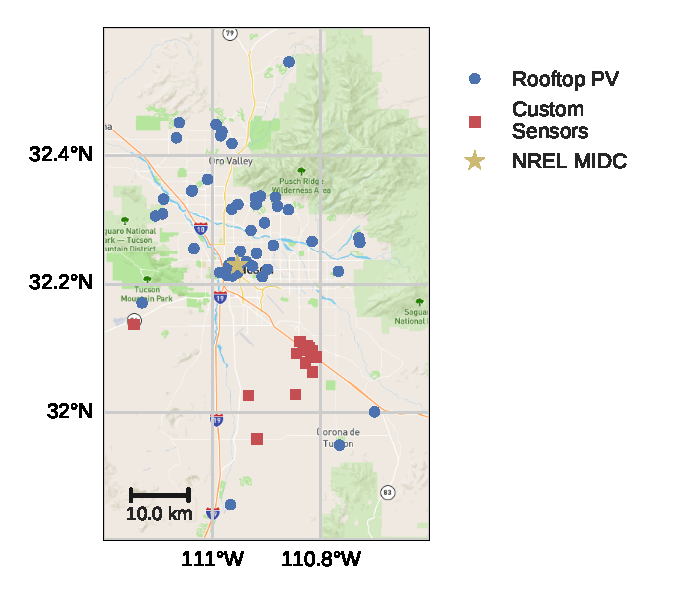
\includegraphics[width=0.75\textwidth]{figs/map.pdf}
\caption[Map of sensor locations]{Map of Tucson, AZ, indicating the
  locations of custom and rooftop PV sensors. The NREL MIDC star
  refers to the calibrated and maintained irradiance sensor located at
  the University of Arizona.}
\label{fig:map}
\end{figure}

The locations of the sensors located in the Tucson, AZ, area are shown
in \cref{fig:map}.
The blue circles denote the locations of rooftop PV systems that we
receive data from as described in \cref{sec:pv_sensors}.
The majority of these sensors are located in central and north Tucson
where the majority of homes are located.
We have no control over the placement of these sensors, but are
grateful to Technicians for Sustainability for setting up the data
transfer and to the homeowners that allow us to use the data.
The time span that data is available depends on each individual
system due to factors such as when it was installed and if the data
transfer stopped for some reason.

The red squares denote the locations of the custom sensors described
in \cref{sec:custom_sensors}.
These sensors were placed south of Tucson where there is a lack of
rooftop PV sensors.
As described in \cref{app:pvsc40}, the primary goal of this
configuration was to study forecasts for a number of PV power plants
located around $32.1^\circ$ N and $110.8^\circ$ W.
The sensors are arranged as they are based on the analysis done in
\cite{Lonij2013}, the fact that the primary cloud direction in
non-monsoon season is from the southwest, and the limited number of
sensors available.
The custom sensors shown in \cref{fig:map} were deployed in late March
2014.
Data from these sensors is available from April to July 2014, when the
sensors started failing due to monsoon rains as mentioned in
\cref{sec:sensor_improvements}.

High-quality 10 second irradiance data has been continuously gathered
from the National Renewable Energy Laboratory (NREL) MIDC OASIS sensor
hosted at the University of Arizona.
This suite of sensors (including GHI and DNI measurements) is part of
the NREL Solar Resource \& Meteorological Assessment Project (SOLRMAP)
and is regularly maintained \citep{Wilcox_Andreas_2010}.
Data from this suite of sensors is publicly available at
\url{http://www.nrel.gov/midc/ua_oasis}.

Data from select sensors in the network supporting
\cite{Lorenzo2015c,Lorenzo2017} is available online
\citep{Lorenzo2015b,Lorenzo2016b}.



%%% Local Variables:
%%% mode: latex
%%% TeX-master: "dissertation"
%%% End:
